%%%%%%%%%%%%%%%%%%%%%%%%%%%%%%%%%%%%%%%%%%%%%%%%%%%%%%%%%%%%%%%%%%%%%%
% LaTeX Example: Project Report
%
% Source: http://www.howtotex.com
%
% Feel free to distribute this example, but please keep the referral
% to howtotex.com
% Date: March 2011 
% 
%%%%%%%%%%%%%%%%%%%%%%%%%%%%%%%%%%%%%%%%%%%%%%%%%%%%%%%%%%%%%%%%%%%%%%
% How to use writeLaTeX: 
%
% You edit the source code here on the left, and the preview on the
% right shows you the result within a few seconds.
%
% Bookmark this page and share the URL with your co-authors. They can
% edit at the same time!
%
% You can upload figures, bibliographies, custom classes and
% styles using the files menu.
%
% If you're new to LaTeX, the wikibook is a great place to start:
% http://en.wikibooks.org/wiki/LaTeX
%
%%%%%%%%%%%%%%%%%%%%%%%%%%%%%%%%%%%%%%%%%%%%%%%%%%%%%%%%%%%%%%%%%%%%%%
% Edit the title below to update the display in My Documents
%\title{Project Report}
%
%%% Preamble
\documentclass[paper=a4, fontsize=11pt]{scrartcl}
\usepackage[T1]{fontenc}
\usepackage{fourier}

\usepackage[english]{babel}															% English language/hyphenation
\usepackage[protrusion=true,expansion=true]{microtype}	
\usepackage{amsmath,amsfonts,amsthm} % Math packages
\usepackage[pdftex]{graphicx}	
\usepackage{url}
\usepackage{titlesec}
\usepackage{listings}
\usepackage{graphicx}


%%% Custom headers/footers (fancyhdr package)
\usepackage{fancyhdr}
\pagestyle{fancyplain}
\fancyhead{}											% No page header
\fancyfoot[L]{}											% Empty 
\fancyfoot[C]{}											% Empty
\fancyfoot[R]{\thepage}									% Pagenumbering
\renewcommand{\headrulewidth}{0pt}			% Remove header underlines
\renewcommand{\footrulewidth}{0pt}				% Remove footer underlines
\setlength{\headheight}{13.6pt}
\usepackage[margin=0.5in]{geometry}

%%% Equation and float numbering
\numberwithin{equation}{section}		% Equationnumbering: section.eq#
\numberwithin{figure}{section}			% Figurenumbering: section.fig#
\numberwithin{table}{section}				% Tablenumbering: section.tab#

%% Section Format
\titleformat*{\section}{\LARGE\bfseries}
\titleformat*{\subsection}{\Large\bfseries}
\titleformat*{\subsubsection}{\large\bfseries}
\titleformat*{\paragraph}{\large\bfseries}
\titleformat*{\subparagraph}{\large\bfseries}


%%% Maketitle metadata
\newcommand{\horrule}[1]{\rule{\linewidth}{#1}} 	% Horizontal rule

\title{
		%\vspace{-1in} 	
		\usefont{OT1}{bch}{b}{n}
		\normalfont \normalsize \textsc{University of Purdue\\
      Data Communication and Computer Networks\\
      CS 53600 Fall 2019} \\ [25pt]
		\horrule{0.5pt} \\[0.4cm]
		\huge Assignment 3\\
		\horrule{2pt} \\[0.5cm]
}
\author{
		\normalfont\normalsize Pedro da Costa Abreu Júnior\\ [-5pt]
    \normalsize Student ID 0030878383\\[-5pt]
    \normalsize \today
}
\date{}


%%% Begin document
\begin{document}
\maketitle

\section{Exercise 2 Discussions}
My first idea to solve the matching problem was the following:
If the client does not receives an ACK then we store that message
timestamp and the sequence number in a variable, and when we receive
that ACK we see if the sequence number matches. But this can
match the wrong ACK with same sequence number.

In order to solve this problem my implementation adds the timestamp
to the header of the communication, so that the ACK can send the timestamp
back, this way we guarantee that the correct ACK will be matched.

For this I created the following new structs (and they can be found in ``utils.h''):

\begin{lstlisting}
typedef struct ack {
  int seqno;
  struct timeval timestamp;
} ack_t;

typedef struct packet {
  int seqno;
  struct timeval timestamp;
  char buf[1343];
} packet_t;
\end{lstlisting}

Notice that we had to shrink the max size of the buffer due to this new
timestamp. Since timeval has the size of two longs, in the worse case scenario
it will be 128 bytes. Since the buffer max size is originally 1471, 1471-128 = 1343.

\section{Exercise 3 Discussions}
Using a file size of 300 and a blocksize of 30 we analyzed the
output of \texttt{tcpdumpwrap-veth0} with \texttt{wireshark}.

Running \textit{ifconfig -a} on the receiver we get:
\begin{lstlisting}
veth0: flags=4163<UP,BROADCAST,RUNNING,MULTICAST>  mtu 1500
        inet 192.168.1.1  netmask 255.255.255.0  broadcast 192.168.1.255
        inet6 fe80::ec4d:4dff:fec2:a2be  prefixlen 64  scopeid 0x20<link>
        ether ee:4d:4d:c2:a2:be  txqueuelen 1000  (Ethernet)
        RX packets 53193  bytes 12742360 (12.7 MB)
        RX errors 0  dropped 0  overruns 0  frame 0
        TX packets 696  bytes 66976 (66.9 KB)
        TX errors 0  dropped 0 overruns 0  carrier 0  collisions 0
\end{lstlisting}

This shows that the mac address of the file sender is \texttt{ee:4d:4d:c2:a2:be}

And running \textit{veth 'ifconfig -a'} on the sender we get:
\begin{lstlisting}
veth0: flags=4163<UP,BROADCAST,RUNNING,MULTICAST>  mtu 1500
        inet 192.168.1.2  netmask 255.255.255.0  broadcast 192.168.1.255
        inet6 fe80::2c5b:78ff:fe7c:1de4  prefixlen 64  scopeid 0x20<link>
        ether 2e:5b:78:7c:1d:e4  txqueuelen 1000  (Ethernet)
        RX packets 696  bytes 66976 (66.9 KB)
        RX errors 0  dropped 0  overruns 0  frame 0
        TX packets 53193  bytes 12742360 (12.7 MB)
        TX errors 0  dropped 0 overruns 0  carrier 0  collisions 0
\end{lstlisting}

This shows that the mac address of the file receiver is \texttt{2e:5b:78:7c:1d:e4}

Here is the byte output of the first message:
\begin{lstlisting}
ee 4d 4d c2 a2 be 2e 5b 78 7c 1d e4 08 00 45 00
00 3b 50 4a 40 00 40 11 67 14 c0 a8 01 02 c0 a8
01 01 82 e9 ec 96 00 27 83 8c 00 33 33 33 33 33
33 33 33 33 33 33 33 33 33 33 33 33 33 33 33 33
33 33 33 33 33 33 33 33 33
\end{lstlisting}

From this we can see that the first 6 bytes is the file receiver mac address
as captured by \texttt{ifconfig}.
The following 6 bytes is the file sender mac address, as captured by \textit{veth 'ifconfig'}.
The following 2 bytes (08 00) is the type of the connection, in this case IPv4.
In the middle of the packet we have 20 bytes of IP header and 8 bytes of UDP header.
Then at the end of the packet we have 00 33 33 ... which is the payload of the communication.
00 is the sequence number and 0x33 is the ascii code for '3'. And we have exactly 30 '3's, as expected.

Now this is the byte output of the second message:
\begin{lstlisting}
2e 5b 78 7c 1d e4 ee 4d 4d c2 a2 be 08 00 45 00
00 1d 1f 7c 40 00 40 11 98 00 c0 a8 01 01 c0 a8
01 02 b8 85 82 e9 00 09 83 6e 00
\end{lstlisting}

Similarly we have the file sender mac address as the 6 bytes and the file receiver mac address as the following 6 bytes.
The last byte (00) is the ACK of the first message (00).


The following was the last two messages with sequence number 2,
ending the communication.

\begin{lstlisting}
ee 4d 4d c2 a2 be 2e 5b 78 7c 1d e4 08 00 45 00
00 1d 50 56 40 00 40 11 67 26 c0 a8 01 02 c0 a8
01 01 82 e9 ec 96 00 09 83 6e 02
\end{lstlisting}

\begin{lstlisting}
2e 5b 78 7c 1d e4 ee 4d 4d c2 a2 be 08 00 45 00
00 1d 1f 86 40 00 40 11 97 f6 c0 a8 01 01 c0 a8
01 02 b8 85 82 e9 00 09 83 6e 02              
\end{lstlisting}

As we can see we have exactly the same message header as before
with the difference that the last byte is 2 for the sequence number ending the communication.

Also notice that in our case padding was not applied in any of the payloads.

\begin{figure}[h]
  \centering
  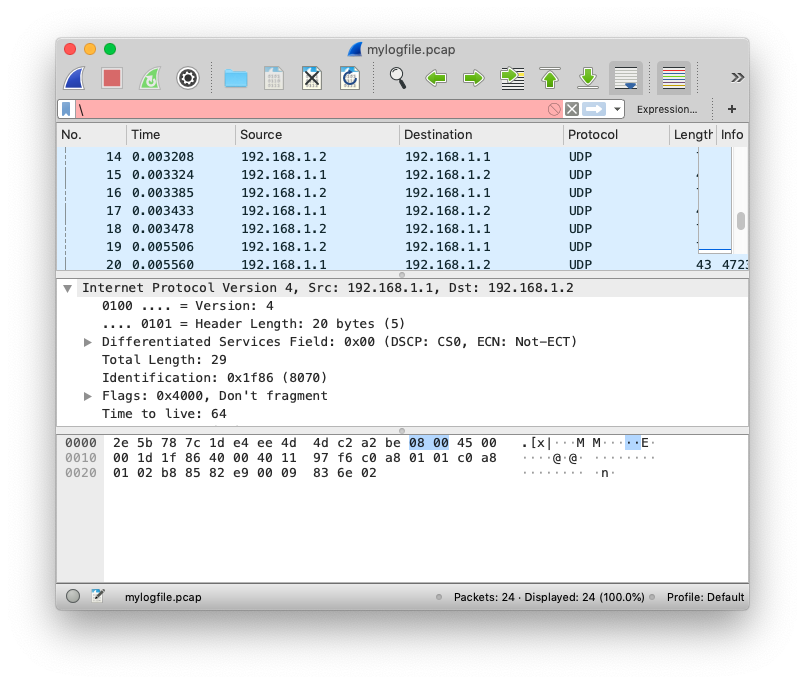
\includegraphics[width=\textwidth]{wireshark}
  \caption{Screenshot of wireshark with the communication log}
\end{figure}

%%% End document
\end{document}
